\documentclass{article}
\usepackage{../fasy-hw}
\usepackage{ wasysym }

%% UPDATE these variables:
\renewcommand{\hwnum}{6}
\title{Advanced Algorithms, Homework \hwnum}
\author{Nathan Stouffer}
\collab{n/a}
\date{due: 26 October 2020}

\begin{document}

\maketitle

In any question that you are expected to provide an algorithm, you are
expected to provide:
\begin{enumerate}
    \item Describe the problem in your own words, including describing what the input and output is.
    \item Describe, in paragraph form, the algorithm you propose.
    \item Provide a nicely formatted algorithm to solve the problem.
    \item Use a decrementing function to prove that algorithm terminates OR  Give the runtime with justification.
    \item Prove partial correctness.
    In other words, if there is a loop or recursion, what is the loop/recursion invariant? Provide the proof.
    (Note: you only need to do this for the outer-most loop if there are nested loops).
\end{enumerate}



\nextprob
\collab{n/a}

Walk through Kruskal's algorithm, using the graph in Figure 7.7 (left) of the
textbook.  Label the center vertex $a$, the other red vertex $b$, and the
remainder $c$ through $g$ in counter-clockwise order.  You should use the
union-find data structure, with both ``heuristics.''

\paragraph{Answer}

% ============================================

TODO: your answer goes between these lines

% ============================================

\nextprob
\collab{n/a}

Chapter 3, Question 9 (Palindromes)

A palindrome is any string that is exactly the same as its reversal.
\begin{enumerate}[label=(\alph*)]
    \item Describe and analyze an algorithm to find the length of the longest subsequence of a given string that is also a palindrome.
    \item Describe and analyze an algorithm to find the length of the shortest supersequence of a given string that is also a palindrome.
    \item Any string can be decomposed into a sequence of palindromes.
    Describe and analyze an efficient algorithm to find the smallest number of palindromes that make up a given input string.
    \item Describe and analyze an efficient algorithm to find the largest integer $k$ such that a given string can be split into palindromes of length at least $k$.
    \item Describe and analyze and efficient algorithm to find the number of different ways that a given string can be decomposed into palindromes.
    \item A metapalindrome is a decomposition of a string into a sequence of palindromes, such that the sequence of palindrome lengths is itself a palindrome.
    Describe and analyze an efficient algorithm to find the length of the shortest metapalindrome for a given string.
\end{enumerate}

\paragraph{Answer}

% ============================================

TODO: your answer goes between these lines

% ============================================

\nextprob
\collab{n/a}

Chapter 7, Question 1 (Shortest and Longest Edges in Cycle)

Let $G = (V, E)$ be an arbitrary connected graph with weighted edges.
\begin{enumerate}[label=(\alph*)]
    \item Prove that for any cycle in $G$, the minimum spanning tree of $G$ excludes the maximum-weight edge in that cycle.
    \item Prove or disprove: The minimum spanning tree of $G$ includes the minimum-weight edge in every cycle in $G$.
\end{enumerate}

\paragraph{Answer}

% ============================================

\begin{enumerate}[label=(\alph*)]
    \item We will prove that given a cycle in $G$, the minimum spanning tree of $G$ does not include the maximum-weight edge in that cycle.
    To this end, pick a cycle $C$ and label the maximum-weight edge $e_{max}$.
    Now suppose we have some spanning tree $T$ that includes $e_{max}$.
    Now we show that $T$ is not the minimum spanning tree for $G$. \parspace
    Since $C$ is a cycle, there exists some edge $e \in C$ that is not contained in $T$ (otherwise $T$ would not be a tree) and that connects the same components that $e_{max}$ connects.
    We know that $e \neq e_{max}$ since $e$ is not contained in $T$.
    Then, by definition of $e_{max}$, we must have $weight(e) < weight(e_{max})$.
    Now let $T' = T - e_{max} + e$.
    Certainly the total weight of $T'$ is less than the total weight of $T$.
    If $T'$ is a spanning tree, then $T$ is certainly not the minimum spanning tree.
    $T'$ must be a spanning tree because $e$ connects the same components that $e_{max}$ connects.
    Therefore, $T$ cannot be a minimum spanning tree since another spanning tree of $G$ exists with less weight.
    \item The minimum spanning tree of $G$ does not necessarily have to include the minimum-weight ege in every cycle of $G$.
    Consider the following counterexample:
    \begin{center}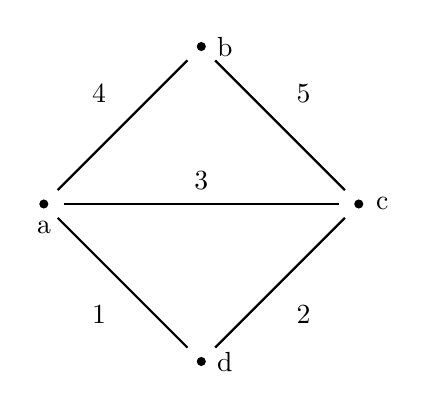
\begin{tikzpicture}[scale=2]
    %% vertices
    \draw [fill=black] (0.0,0.0)     circle (0.025);
    \draw [fill=black] (1.0,1.0)     circle (0.025);
    \draw [fill=black] (2.0,0.0)     circle (0.025);
    \draw [fill=black] (1.0,-1.0)    circle (0.025);
    %% labels
    \node at (0.0,-0.15) {a};
    \node at (1.15,1.0) {b};
    \node at (2.15,0.0) {c};
    \node at (1.15,-1.0) {d};
    %% weights
    \node at (0.35,-0.7) {1};
    \node at (1.65,-0.7) {2};
    \node at (1,0.15) {3};
    \node at (0.35,0.7) {4};
    \node at (1.65,0.7) {5};

    %% edges
    \draw [thick] (0.088,0.088) -- (0.912,0.912);
    \draw [thick] (0.125,0.0) -- (1.875,0.0);
    \draw [thick] (0.088,-0.088) -- (0.912,-0.912);
    \draw [thick] (1.088,0.912) -- (1.912,0.088);
    \draw [thick] (1.912,-0.088) -- (1.088,-0.912);
\end{tikzpicture}
\end{center}
    Consider the cycle $a \to b \to c \to a$ which has minimum-weight edge $ac$.
    But the above graph has minimum spanning tree with edges $ad, dc, ab$.
    The minimum spanning tree does not contain $ac$ so we have found a counterexample.
\end{enumerate}

% ============================================


\nextprob
\collab{n/a}

Chapter 8, Question 3 (Weights on Vertices)

Suppose we are given an undirected graph $G$ in which every vertex has a positive weight.
\begin{enumerate}[label=(\alph*)]
    \item Describe and analyze an algorithm to find a spanning tree of $G$ with minimum total weight.
    \item Describe and analyze an algorithm to find a path in $G$ from one given vertex $s$ to another given vertex $t$ with minimum total weight.
\end{enumerate}

\paragraph{Answer}

% ============================================
\begin{enumerate}[label=(\alph*)]
    \item We first describe and analyze an algorithm to find a spanning tree of $G$ with minimum total weight.
        \begin{enumerate}[label=\alph*)]
            \item The input to the problem is a connected, undirected graph $G = (V, E)$ paired with a weight function $w: V \rightarrow \R ^+$.
            We define the weight of a graph $G$ to be $weight(G) = \sum _{v \in V} w(v)$. \parspace
            The output will be a tree with minimum weight $T = (V_T, E_T) \subset G$ such that every vertex of $V$ is in $T$ and $T$ is connected.
            In this problem, every vertex must be contained in $T$ so the weight of every spanning tree is the same value.
            \item Since every spanning tree of $G$ will have the same weight, we need only provide an algorithm that computes a spanning tree $T$ of $G$.
            To do this, we will use a union-find data structure.
            First, we will initialize the data structure with every vertex in its own component.
            Then we will iterate over every edge.
            For each edge $e = (s, t)$, we will test if $s$ and $t$ are in the same component.
            If not, union them in the data structure and add $e$ to $T$.
            After iterating through the edges, $T$ will be a miminum spanning tree for $G$.
            \item Here is the algorithm:
            \begin{algorithm}
                \textsc{MST}($G = (V, E)$) \\
                1. \hspace{1em} $T = (V, \emptyset)$ \\
                2. \hspace{1em} uf = init($V$) \\
                3. \hspace{1em} for $i=1..|E|$ \\
                4. \hspace{2em}     $(s_i, t_i) = E[i]$ \\
                5. \hspace{2em}     if (uf.find($s_i$) $\neq$ uf.find($t_i$)) \\
                6. \hspace{3em}         uf.union($s_i, t_i$) \\
                7. \hspace{3em}         $T = T \cup (\emptyset, (s_i, t_i)) $       // add edge to tree \\
                8. \hspace{1em} return $T$
            \end{algorithm}
            \item We prove that \textsc{MST} terminates by giving a run time analysis.
            Line 1 takes constant time and line 2 takes $\Theta (V)$ time.
            Line 3 runs exactly $|E|$ times and lines 4, 7, and 8 all run in constant time.
            This leaves only lines 5 and 6 unaccounted for.
            If we use the heuristic version of union find, then both lines run in constant time.
            Therefore the run time of the algorithm is a composition of polynomials, which is finite and the algorithm must terminate.
            \item We now prove partial correctness.
            Suppose that \textsc{MST} terminates, will it terminate in a correct state?
            We will define a loop invariant for the loop beginning on line 3.
            At iteration $i$, the loop invariant $L_i$ is that $T_i$ is a forest of the connected components of $G$ after processing the first $i$ edges.
            Prior to the for loop, we have not processed any edges so $T$ should just contain every vertex in its own connected component, which is the case.
            As we are processing the for loop, an edge is added to $T$ only if the vertices are found to be in different components, thus connecting the components and preserving the forest structure of $T$.
            After the for loop terminates (which we know will occur because we proved termination), we will have processed every edge.
            Then $T$ is not a forest, but a spanning tree since the graph $G$ is assumed to be connected.
            Thus, we return a spanning tree from the \textsc{MST} which must be a minimum spanning tree since every spanning tree has the same total weight.
        \end{enumerate}
    \item Describe and analyze an algorithm to find a path in $G$ from one given vertex $s$ to another given vertex $t$ with minimum total weight.
        \begin{enumerate}[label=\alph*)]
            \item Input and output.
            \item describe algorithm in own words
            \item Provide a nicely formatted algorithm to solve the problem.
            \item Use a decrementing function to prove that algorithm terminates OR  Give the runtime with justification.
            \item Prove partial correctness.
            In other words, if there is a loop or recursion, what is the loop/recursion invariant? Provide the proof.
            (Note: you only need to do this for the outer-most loop if there are nested loops).
        \end{enumerate}
\end{enumerate}

% ============================================




\nextprob
\collab{n/a}

Describe a ``real-life'' problem that can be modeled as:

\begin{enumerate}
    \item An undirected graph.
    \item A directed, weighted graph.
    \item A tree.
    \item A forest.
\end{enumerate}

\paragraph{Answer}

% ============================================

TODO: your answer goes between these lines
% ============================================


\end{document}
